\documentclass[twoside=false,DIV=14]{scrartcl}
\usepackage{arev} % order matters, putting this above allows FiraSans to override it for body text
\usepackage[sfdefault]{FiraSans}
\usepackage{inconsolata}
%\usepackage[fira]{fontsetup}
\usepackage{scrlayer-scrpage}
\renewcommand{\titlepagestyle}{scrheadings}
\usepackage{graphicx}
\usepackage{blindtext}
\usepackage{wrapfig}
\usepackage{tabularx}
\usepackage{hyperref}
\usepackage{listings}
\usepackage{tikz}
\usepackage{amsmath}
\usepackage[many]{tcolorbox}

\usepackage{xcolor,sectsty}
\definecolor{blackish}{RGB}{56,58,54}
\definecolor{redish}{RGB}{109,41,49}
\definecolor{red}{RGB}{152,41,50}
\definecolor{orangeish}{RGB}{188,71,0}
\definecolor{blueish}{RGB}{25,33,139}
\subsubsectionfont{\color{blackish}}
\subsectionfont{\color{blackish}}
\sectionfont{\color{blackish}}

\lohead{\color{red} COMP3000 Programming Languages}
\rohead{
\includegraphics[width=0.5cm]{../logo.jpg}}

\setkomafont{author}{\sffamily \small}
\setkomafont{date}{\sffamily \small}

\DeclareOldFontCommand{\bf}{\normalfont\bfseries}{\mathbf}
\DeclareOldFontCommand{\tt}{\normalfont\ttfamily}{\texttt}

\lstset{basicstyle=\ttfamily}


\date{}
\newtcolorbox{aside}[1][]{
  title=Aside,
  width=0.3\textwidth,
  fonttitle=\bfseries,
  breakable,
  fonttitle=\bfseries\color{black},
  colframe=blueish!80,
  colback=blueish!2
  #1}

\newtcolorbox{note}[1][]{
  title=Note,
  width=\textwidth,
  fonttitle=\bfseries,
  breakable,
  fonttitle=\bfseries\color{black},
  colframe=orangeish!80,
  colback=orangeish!2
  #1}

\newtcolorbox{hint}[1][]{
    title=Hint,
    width=\textwidth,
    fonttitle=\bfseries,
    breakable,
    fonttitle=\bfseries\color{white},
    colframe=blueish!80,
    colback=blueish!2
    #1}

\newtcolorbox{todo}[1][]{
  title=!! TODO !!,
  width=\textwidth,
  fonttitle=\bfseries,
  breakable,
  fonttitle=\bfseries\color{white},
  colframe=red!80,
  colback=red!2
  #1}
  
\providecommand{\tightlist}{%
  \setlength{\itemsep}{0pt}\setlength{\parskip}{0pt}}

\usepackage{caption}
\captionsetup{labelformat=empty}

\title{\color{redish} \vspace{-1em}COMP3000: EPIC Programming Languages}

\begin{document}
{\color{blackish}\maketitle}\vspace{-7em}

\begin{abstract}
\end{abstract}
    Programming Languages is a third-year computing unit which combines \emph{computer science} and \emph{software engineering} and occupies a critical place in the Software Engineering and Software Technology programs of study.  In 2025 it will be taught in an EPIC style which, while a natural fit for engineering units, is not so simply implemented for an applied mathematics like computer science.  


\begin{figure}[h]
    \begin{center}
      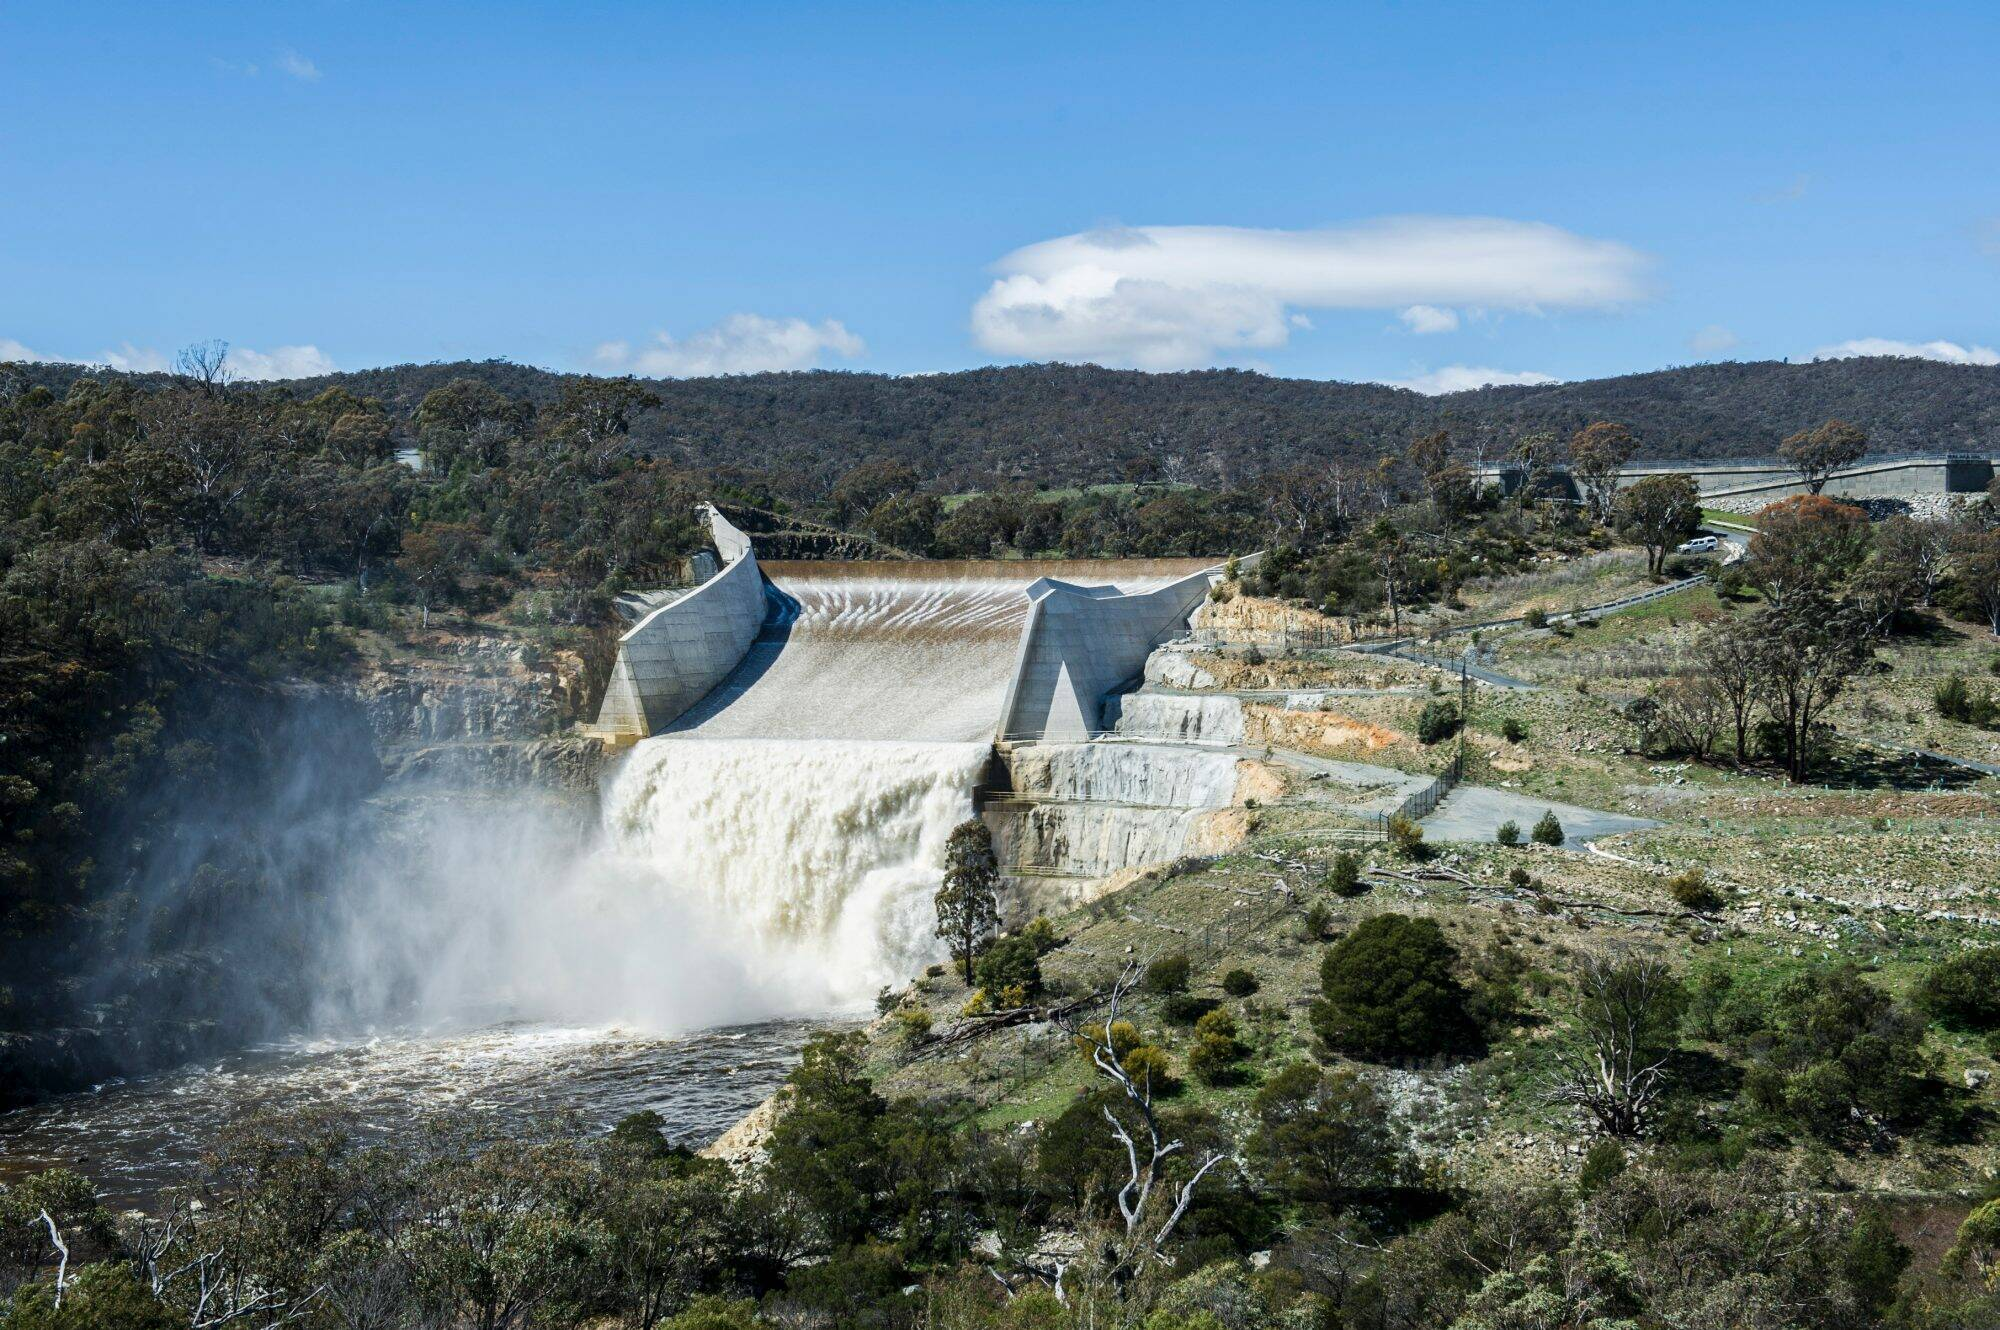
\includegraphics[width=0.8\textwidth]{googong.jpg}
    \end{center}
    \caption{The Googong Dam is one of the river flows students will describe.}
  \end{figure}
  
  
This unit of study is also a \emph{content-heavy} unit with many complex concepts that need mastering to complete the learning outcomes.  In this document we describe this unit of study at a high level and show how content-heavy units can be an EPIC experience.

\begin{description}
\item[Experience that transforms] One of the career paths for students completing this unit is to join specialised software consultancies that help clients solve particularly difficult problems which normal consultancies have failed to solve and that is exactly what the students will experience in this unit of study.
\item[Purpose that inspires] The classwork will guide students through the task of creating a unique programming language with novel, real-world applications.  The students will see that the capability they are creating does not yet exist and will see how their work can fill that hole in the real world for a real client.  
\item[Impact that matters] In 2025 the classwork will revolve around creating a \emph{language} to model water flows in river systems.  While simulation-based approaches already exist, language-based solutions do not.  Language-based solutions require specific skills (those covered in this unit of study) which are not widely available but in return are more powerful, more flexible, more understandable, and more maintainable.  Each group will create their own such language and will demonstrate the value of it to interested parties.  The student's work won't match the feature set of existing simulation-based products, but will demonstrate the potential for language-based solutions to supplant them.
\item[Collaboration that empowers] Classes are organised around \emph{Team Based Learning}.  Students work in teams on carefully calibrated activities which both re-inforce the fundamental concepts/skills \emph{and} allows them to creatively apply them as they choose.  There will be thirteen 2-hour collaborative classes accross semester at convenient times for students to choose from.  Students will form groups in the first week and work in those groups throughout all thirteen classes.
\end{description}

\begin{figure}[h]
    \begin{center}
    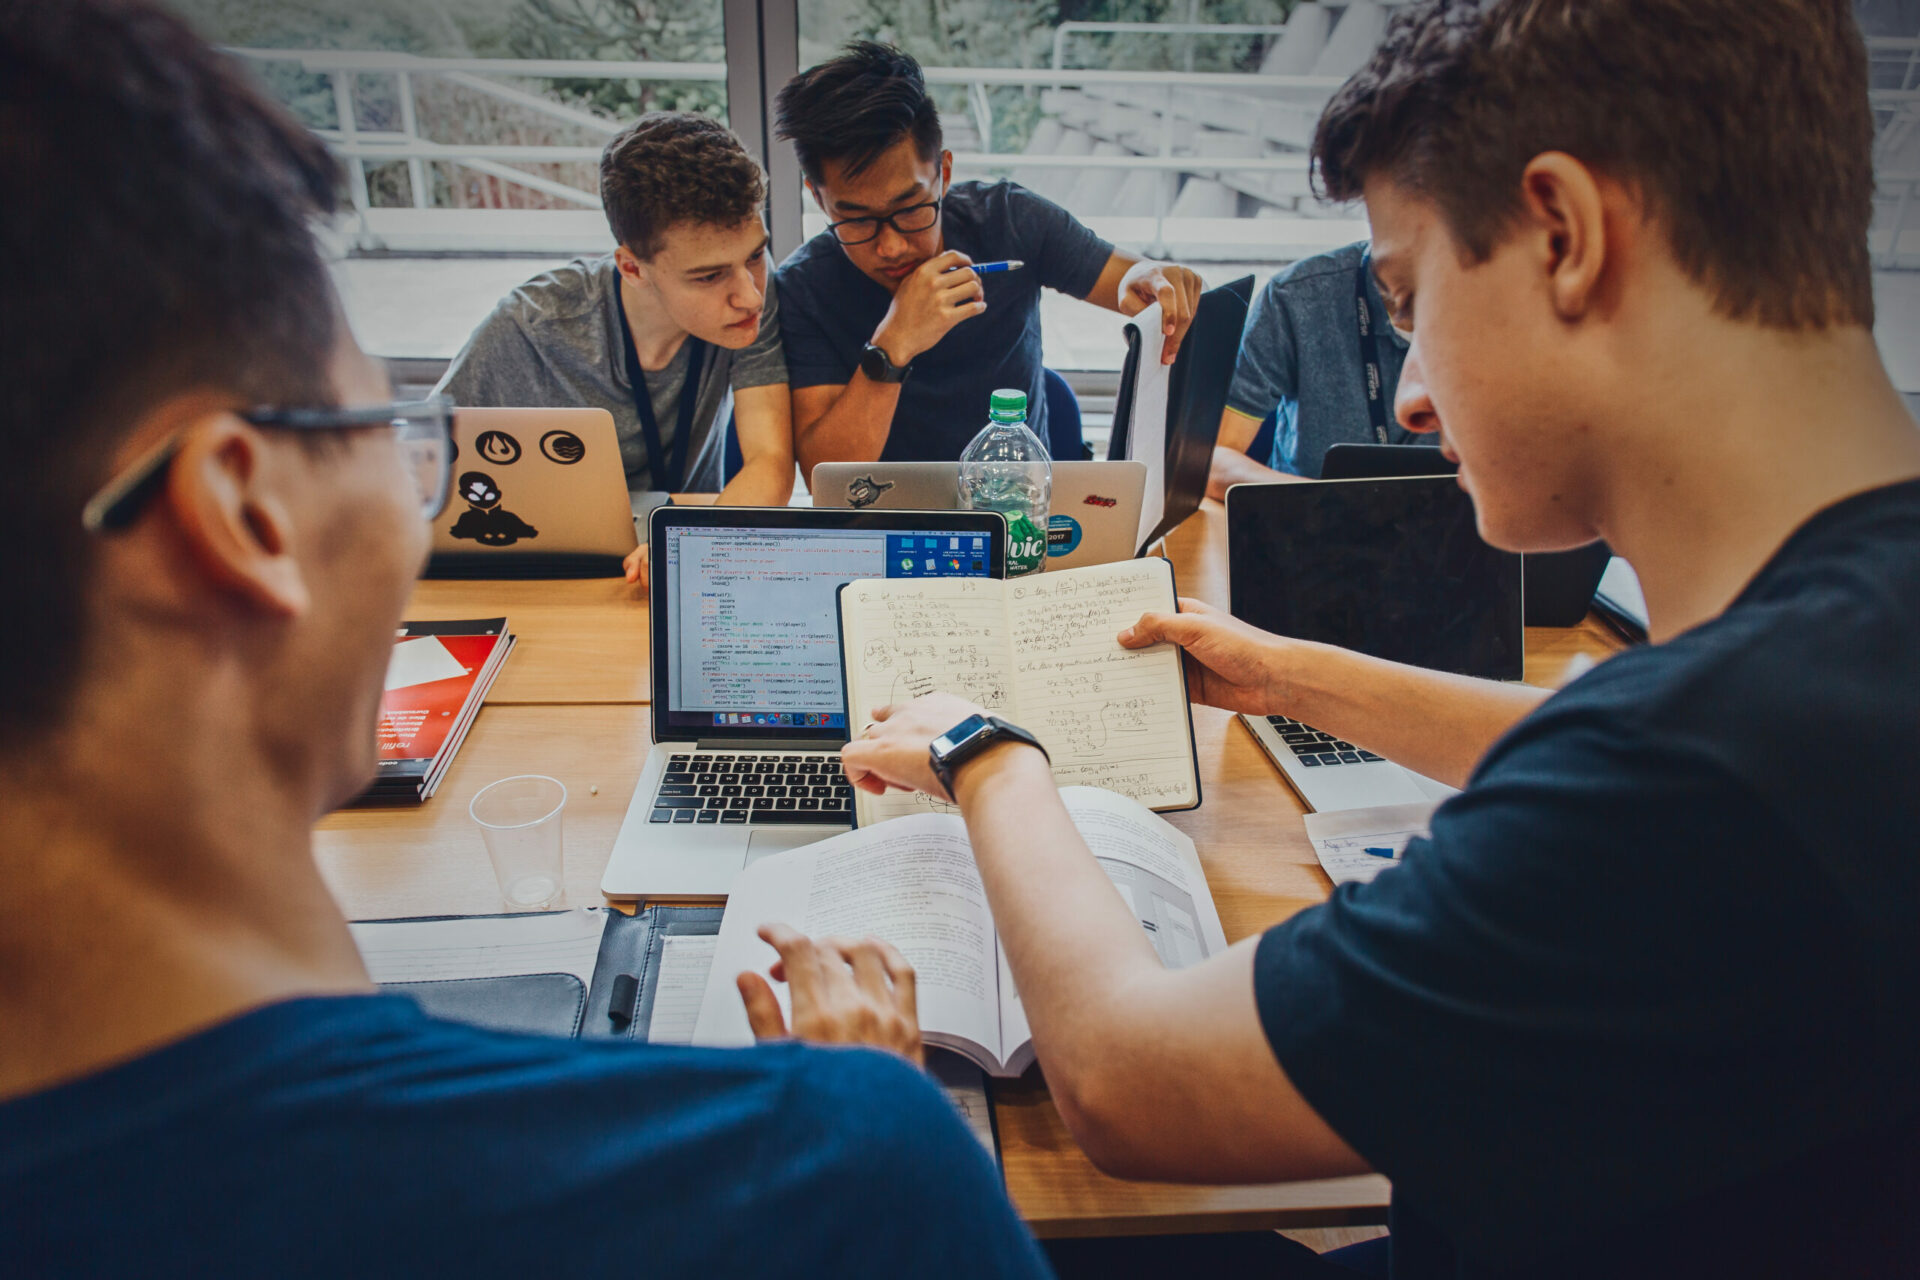
\includegraphics[width=0.8\textwidth]{tbl.jpg}
\end{center}
\caption{Students will work collaboratively in all classes, acting as a specialist consultancy}
\end{figure}

\begin{tabular}{lcl}
\textbf{class \#} & \textbf{content and skills} & \textbf{EPIC activities} \\
\hline
1 & team based learning  & creating effective teams\\
2 & little languages & regular expression upskill \\
3 & lox & generating code for a graphics language from lox \\
4 & scanning & teamwork skills for consultant programmers \\
5 & abstract syntax trees and grammars & a simple language of water flows\\
6 & parsing grammars & parsing representations of water flows \\
7 & evaluation of expressions & computing water flows \\
8 & statements & exploration of student ideas \\
9 & statements & how variables lift expressiveness\\
10 & control flow & water flow managements with Dams \\
11 & functions & unlocking full power with functions \\
12 & functions & crafting a demonstration \\
13 & resolving & exploration of student ideas \\
\hline
\end{tabular}

\end{document}

